\documentclass[a4paper]{article}
\usepackage[utf8x]{inputenc}
\usepackage[T1,T2A]{fontenc}
\usepackage[russian]{babel}
\usepackage{hyperref}
\usepackage{indentfirst}
\usepackage{listings}
\usepackage{color}
\usepackage{here}
\usepackage{array}
\usepackage{multirow}
\usepackage{graphicx}
\usepackage{caption}
\graphicspath{{graphics/}}
\usepackage[left=2cm,right=2cm,
top=2cm,bottom=2cm,bindingoffset=0cm]{geometry}
\usepackage{listings}
\lstset{ %
	extendedchars=\true,
	keepspaces=true,
	language=bash,					% choose the language of the code
	basicstyle=\footnotesize,		% the size of the fonts that are used for the code
	numbers=left,					% where to put the line-numbers
	numberstyle=\footnotesize,		% the size of the fonts that are used for the line-numbers
	stepnumber=1,					% the step between two line-numbers. If it is 1 each line will be numbered
	numbersep=5pt,					% how far the line-numbers are from the code
	backgroundcolor=\color{white},	% choose the background color. You must add \usepackage{color}
	showspaces=false				% show spaces adding particular underscores
	showstringspaces=false,			% underline spaces within strings
	showtabs=false,					% show tabs within strings adding particular underscores
	frame=single,           		% adds a frame around the code
	tabsize=2,						% sets default tabsize to 2 spaces
	captionpos=b,					% sets the caption-position to bottom
	breaklines=true,				% sets automatic line breaking
	breakatwhitespace=false,		% sets if automatic breaks should only happen at whitespace
	escapeinside={\%*}{*)},			% if you want to add a comment within your code
	postbreak=\raisebox{0ex}[0ex][0ex]{\ensuremath{\color{red}\hookrightarrow\space}}
}

\begin{document}	% начало документа

\begin{titlepage}	% начало титульной страницы

	\begin{center}		% выравнивание по центру

		\large Санкт-Петербургский Политехнический Университет Петра Великого\\
		\large Институт компьютерных наук и технологий \\
		\large Кафедра компьютерных систем и программных технологий\\[6cm]
		% название института, затем отступ 6см
		
		\huge Телекоммуникационные технологии\\[0.5cm] % название работы, затем отступ 0,5см
		\large Отчет по лабораторной работе №4 \\[0.2cm]
		\large\textbf{"Аналоговая модуляция"}\\[5cm]

	\end{center}


	\begin{flushright} % выравнивание по правому краю
		\begin{minipage}{0.25\textwidth} % врезка в половину ширины текста
			\begin{flushleft} % выровнять её содержимое по левому краю

				\large\textbf{Работу выполнил:}\\
				\large Вотчицев К. В.\\
				\large {Группа:} 33501/3\\
				
				\large \textbf{Преподаватель:}\\
				\large Богач Н.В.\

			\end{flushleft}
		\end{minipage}
	\end{flushright}
	
	\vfill % заполнить всё доступное ниже пространство

	\begin{center}
	\large Санкт-Петербург\\
	\large \the\year % вывести дату
	\end{center} % закончить выравнивание по центру

\thispagestyle{empty} % не нумеровать страницу
\end{titlepage} % конец титульной страницы

\vfill % заполнить всё доступное ниже пространство

\section{Цель работы}
Изучение амплитудной модуляции/демодуляции сигнала.

\section{Постановка задачи}
\begin{itemize}
	\item Сгенерировать однотональный сигнал низкой частоты.
	\item Выполнить амплитудную модуляцию (АМ) сигнала по закону $u(t)=(1+MU_mcos(\Omega t))+cos(\omega_0t+\phi_0)$ для различных значений глубины модуляции M. Используйте встроенную функцию
	MatLab ammod.
	\item Получить спектр модулированного сигнала.
	\item Выполнить модуляцию с подавлением несущей $u(t)=MU_mcos(\Omega t)cos(\omega_0 t+\phi_0)$. Получить спектр.
	\item  Выполнить однополосную модуляцию:
		
	$U(t)=U_mcos(\Omega t)cos(\omega_0t+\phi_0)+\frac{U_m}{2}\sum_{n=1}^{N}M_n(cos(\omega_0+\Omega_n)t+\phi_0+\Phi_0)$, положив n=1.
	\item Выполнить синхронное детектирование и получить исходный однополосный сигнал
	\item Рассчитать КПД модуляции
	
	$\eta_AM=\frac{U_m^2M^2/4}{P_U}=\frac{M^2}{M^2+2}$
\end{itemize}


\section{Теоретический раздел}
Для передачи по любому каналу связи цифровое сообщение, представляющее собой последовательность символов (чисел), необходимо преобразовать в аналоговый сигнал - изменяющуюся во времени физическую величину (например, напряжение). Кроме того, канал связи способен пропускать лишь определенную полосу частот. Преобразование сигнала для переноса в заданный частотный диапазон осуществляется путем модуляции. Обратный процесс назвается демодуляцией.\\

Амплитудная модуляция - вид модуляции, при которой изменяемым параметром несущего сигнала является его амплитуда. Простейшая форма модулированного сигнала создается при однотональной амплитудной модуляции - модуляцией несущего сигнала гармоническим колебанием с одной частотой $\omega$.\\

$u(t)=(1+MU_mcos(\Omega t))+cos(\omega_0t+\phi_0)$\\

Коэффициент полезного действия модуляции определяется по формуле:\\

$\eta_AM=\frac{U_m^2M^2/4}{P_U}=\frac{M^2}{M^2+2}$\\

Модуляция с подавлением несущей частоты - вид модуляции, при которой происходит подавление несущего колебания, что делает КПД модуляции равным 100\%. Модуляция с подавлением несущей выполняется по закону:\\

$U(t)=U_mcos(\Omega t)cos(\omega_0t+\phi_0)+\frac{U_m}{2}\sum_{n=1}^{N}M_n(cos(\omega_0+\Omega_n)t+\phi_0+\Phi_0)$\\

\section{Ход работы}
Сгенерируем однотональный сигнал низкой частоты.
\captionof{lstlisting}{Генерация модулирующего сигнала}
\lstinputlisting[firstline=4, lastline=13]{../lab4.m}
\begin{center}
	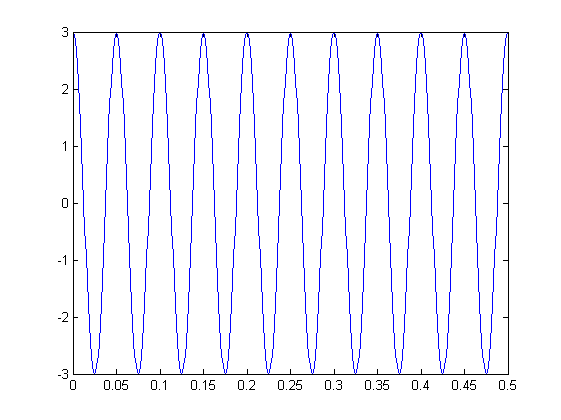
\includegraphics[scale = 0.7]{sign.png} \\Рис.1 Модулирующий сигнал
\end{center}

Выполним амплитудную модуляцию, используя функцию ammod.
\captionof{lstlisting}{Амплитудная модуляция}
\lstinputlisting[firstline=15, lastline=21]{../lab4.m}
\begin{center}
	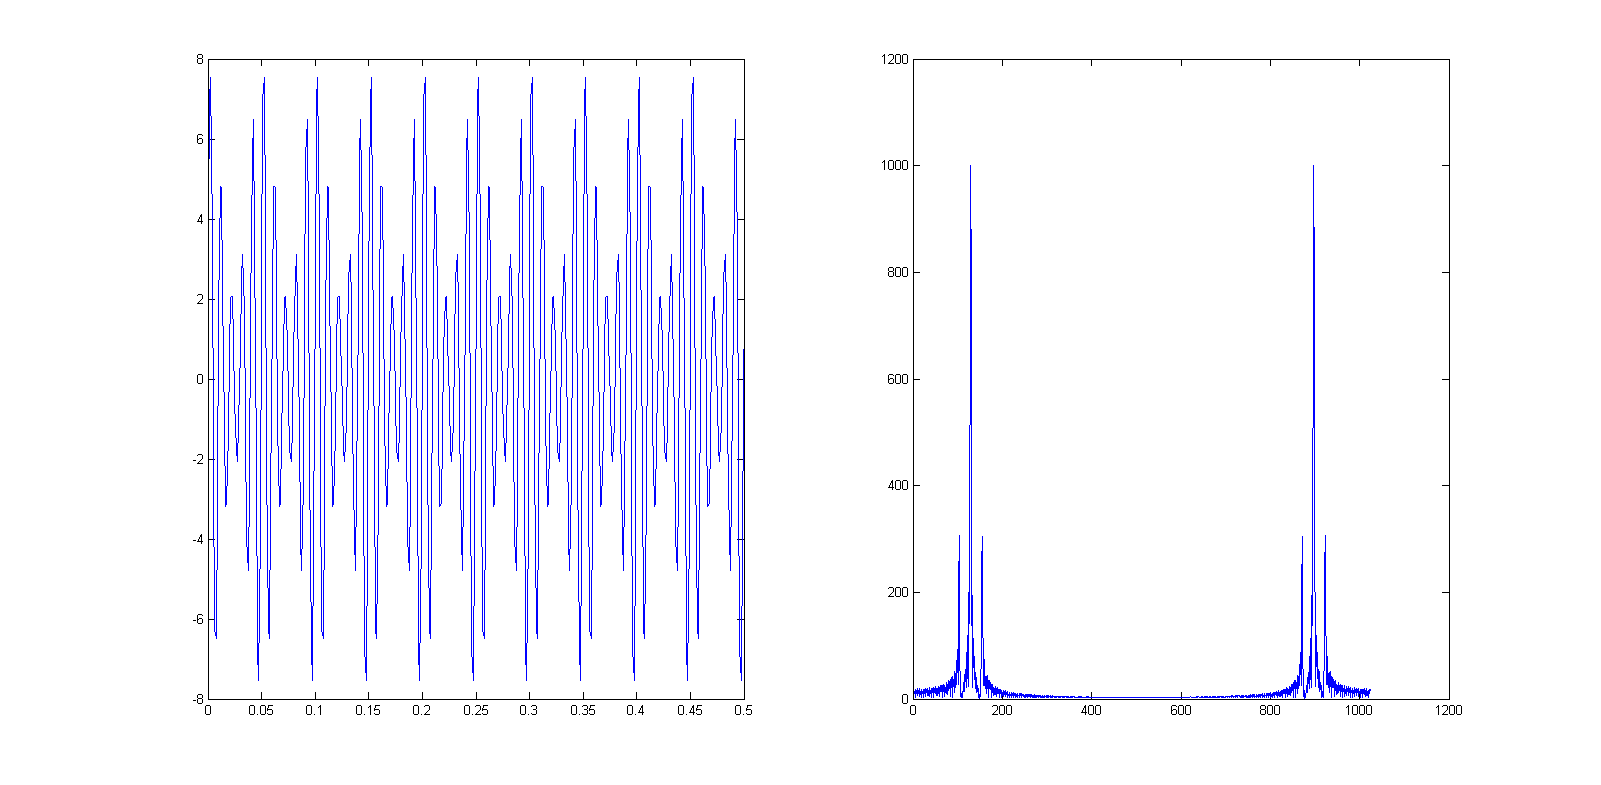
\includegraphics[scale = 0.4]{ammod.png} \\Рис.2 Амплитудная модуляция
\end{center}

Выполним модуляцию с подавлением несущей.
\captionof{lstlisting}{Модуляция с подавлением несущей}
\lstinputlisting[firstline=23, lastline=29]{../lab4.m}
\begin{center}
	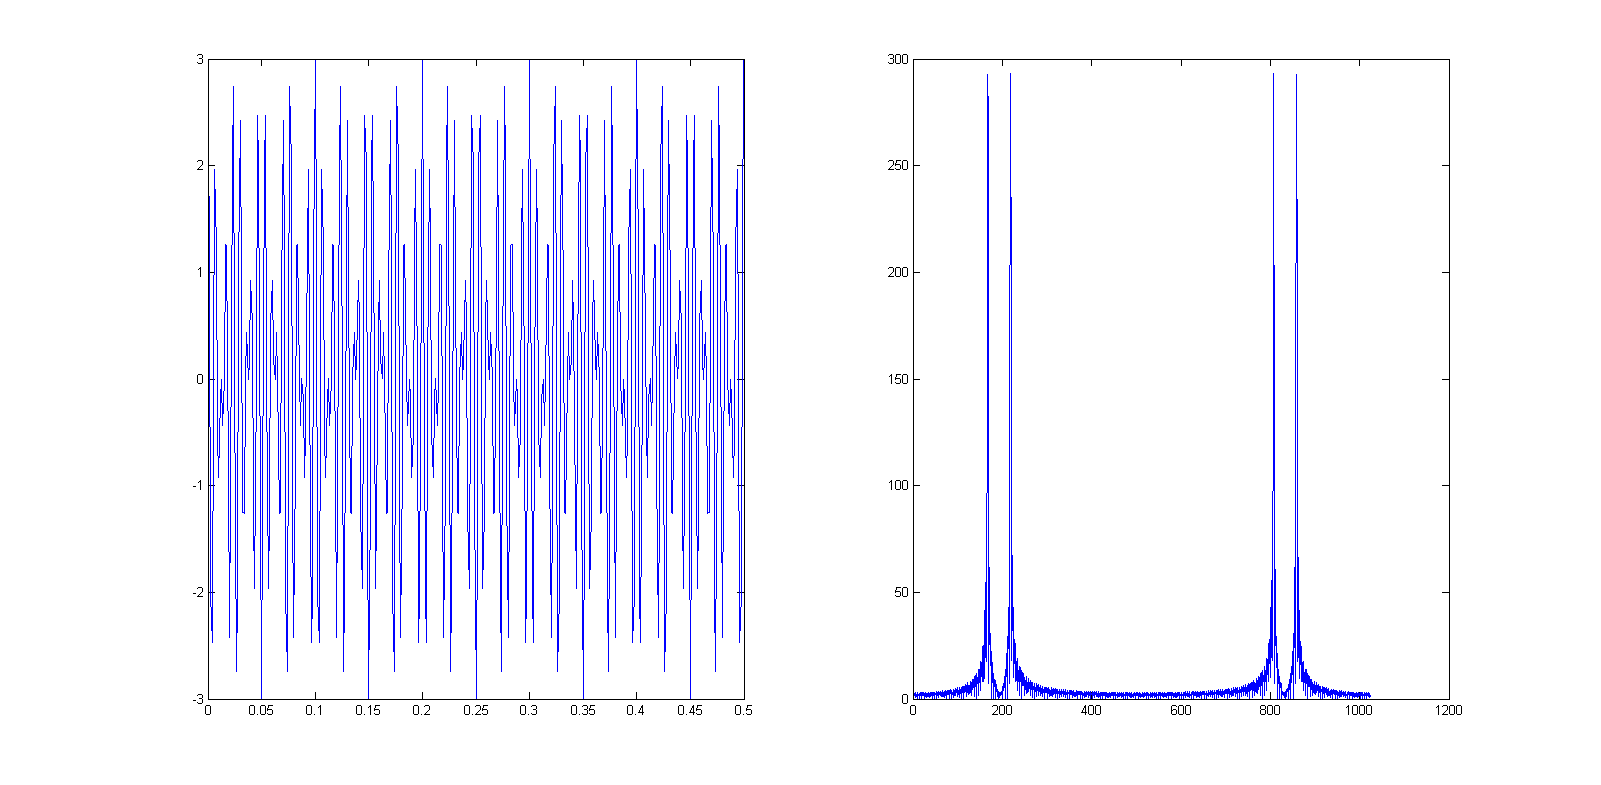
\includegraphics[scale = 0.4]{sub_mod.png} \\Рис.3 Модуляция с подавлением несущей
\end{center}

Выполним однополосную модуляцию, используя функцию ssbmod.
\captionof{lstlisting}{Однополосная модуляция}
\lstinputlisting[firstline=31, lastline=36]{../lab4.m}
\begin{center}
	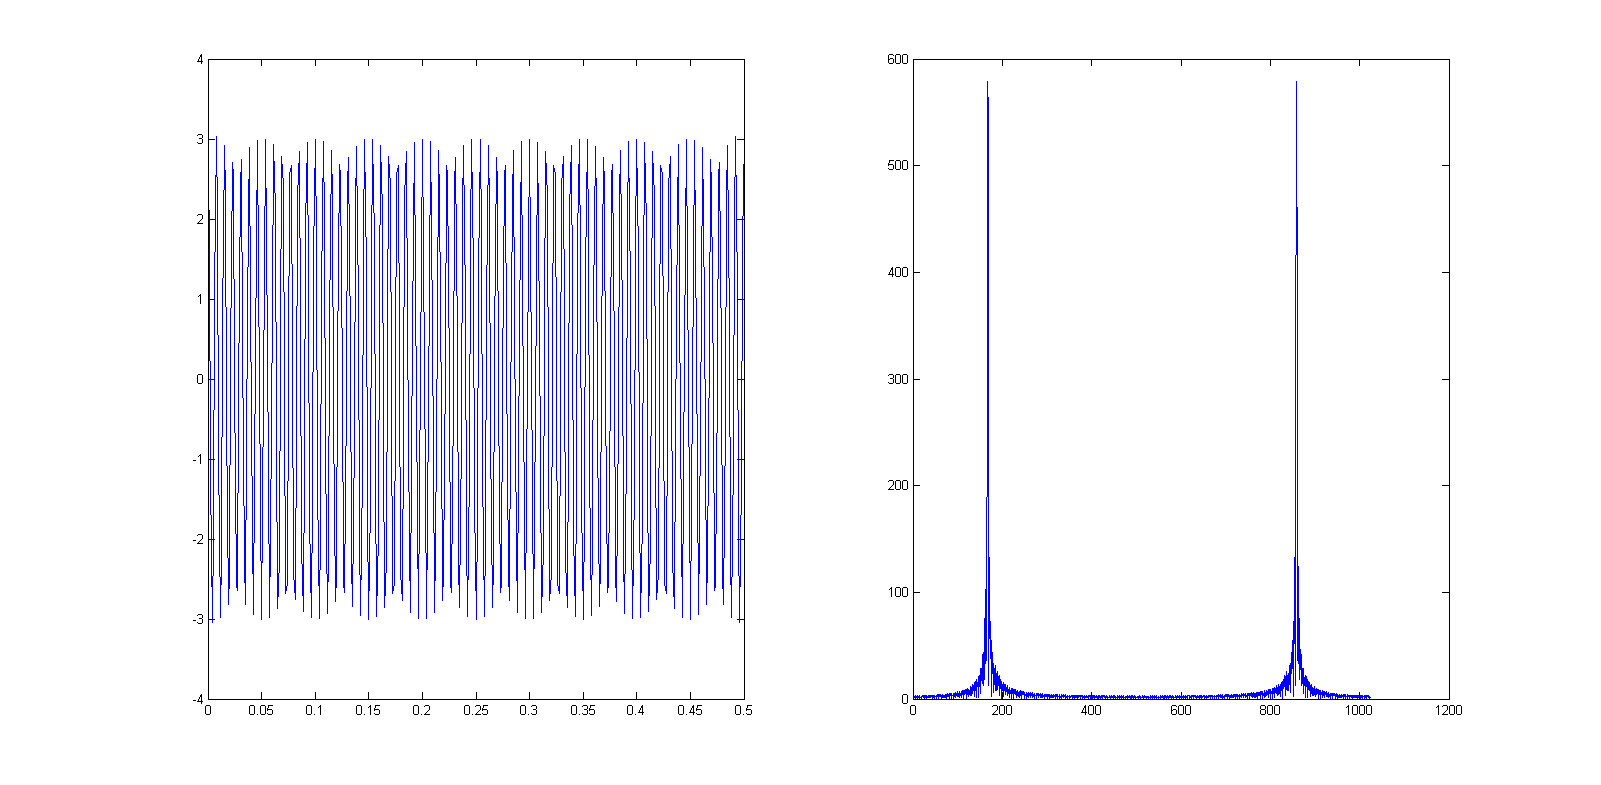
\includegraphics[scale = 0.4]{single_mod.png} \\Рис.4 Однополосная модуляция
\end{center}

Выполним синхронное детектирование и получим исходный однополосный сигнал.
 \captionof{lstlisting}{Синхронное детектирование}
 \lstinputlisting[firstline=38, lastline=43]{../lab4.m}
 \begin{center}
 	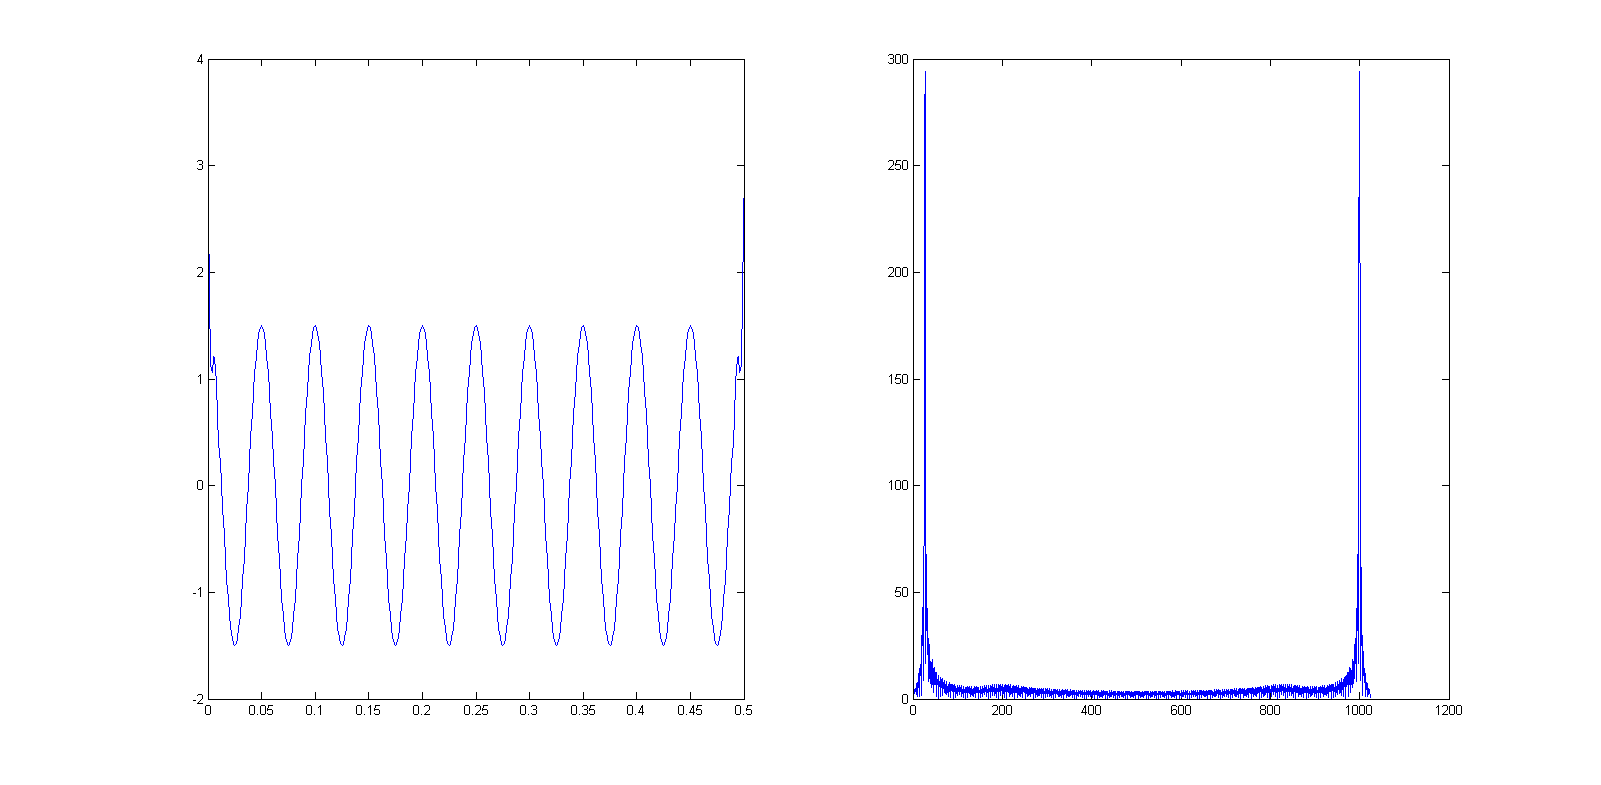
\includegraphics[scale = 0.4]{demod.png} \\Рис.5 Сигнал после синхронного детектирования
 \end{center}

Найдем КПД амплитудной модуляции.
 \captionof{lstlisting}{Расчет КПД}
\lstinputlisting[firstline=45, lastline=46]{../lab4.m}

КПД = 0.15

\section{Выводы}
В ходе выполнения лабораторной работы исследована амплитудная модуляция/демодуляция сигнала. Без подавления несущей при М<1 основная мощность передаваемого информационного сигнала намного меньше мощности несущего колебания, поэтому амплитудная модуляция имеет низкий КПД. При подавлении несущей КПД модуляции равно 100\%.
\end{document}



